

  \begin{itemize}
    \item A signal is $x(t)$ a function of time, an image $x(\v)$ a function of space.
    \item Those functions are what we measure/observe  but can be hard to
    interpret/process automatically.
    \item Another representation for a signal is in the frequency domain ($1/t$).
    \item Better representation for numerous applications.
  \end{itemize}


  \begin{exampleblock}{Applications}
    \begin{itemize}
      \item Signal processing (biomedical, electrical).
      \item Image processing (2D signals), filtering, reconstruction.
      \item Colors are combination of waves of different frequencies.
    \end{itemize}
  \end{exampleblock}
  
\section{Fourier series}
\label{sec:fourier-transform}



\begin{center}
    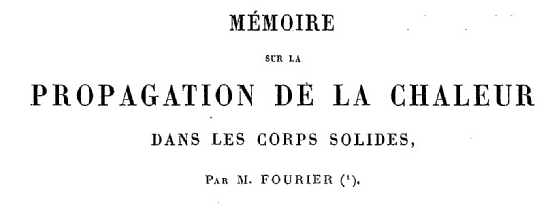
\includegraphics[width=.7\linewidth]{imgs/fourier/fourier_series_title}
    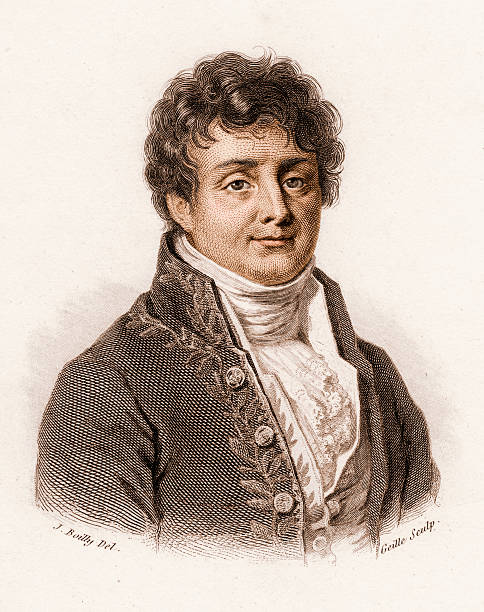
\includegraphics[width=.2\linewidth]{imgs/fourier/fourier}

    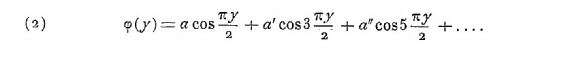
\includegraphics[width=.7\linewidth]{imgs/fourier/fourier_series1}
    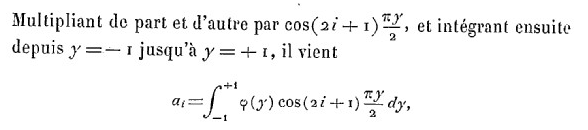
\includegraphics[width=.7\linewidth]{imgs/fourier/fourier_series2}
  \end{center}
  \vspace{-5mm}
  \begin{block}{History}
    \begin{itemize}
      \item Trigonometric series used by Euler, d'Alembert, Bernoulli and Gauss.
      \item Introduced by Joseph Fourier in \cite{fourier1807memoire}.
      \item Fourier claimed that these series could approximate any function.
    \end{itemize}

  \end{block}


  \begin{block}{Decomposition as trigonometric series}
    One can express periodic $x(t)$ of period $T_0=\frac{2\pi}{w_0}$ integrable on the period as
$$
x(t)= \frac{a_0}{2} + \sum_{k=1}^\infty \left [a_k \cos (k w_0 t) +
  b_k \sin (k w_0 t) \right]
$$

where $a_k$ and $b_k$ are the Fourier coefficients that can be computed as
$$
a_k = \frac{2}{T_0} \int_{T_0} x(t) \cos (k w_0 t) dt \quad \quad b_k
= \frac{2}{T_0} \int_{T_0} x(t) \sin (k w_0 t) dt
$$

\begin{itemize}
  \item Representation of a periodic signal as an infinite number of coefficients corresponding to harmonic frequencies.
  \item Can be interpreted as a change of basis from temporal to frequencies.
  \item Functions can be approximated with a finite number $N$ of terms.
  \item Gibbs phenomenon appears for discontinuous functions \cite{hewitt1979gibbs}.
\end{itemize}

\end{block}


\begin{figure}[t]
    \centering
    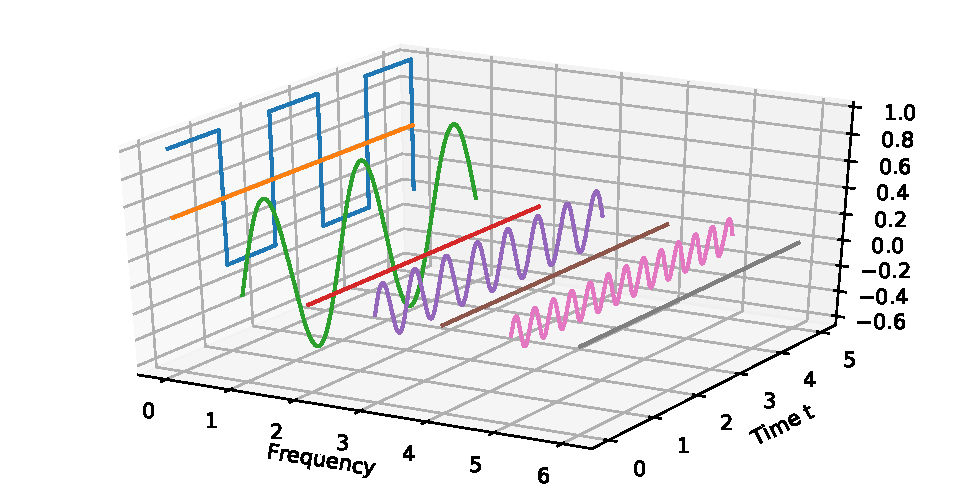
\includegraphics[width=.64\linewidth]{imgs/fourier/fourier_series_3d}
    \caption{Illustration of Fourier series for Example }
    \label{fig:label}
\end{figure}

\begin{exampleblock}{Example : Square wave}
    \begin{columns}
      \begin{column}{5cm}
        \begin{itemize}
        \item Square wave with $T_0=2$
  %$$x(t)=\sum_{k=-\infty}^\infty \Pi_T(t-\frac{T}{2}-kT)$$

      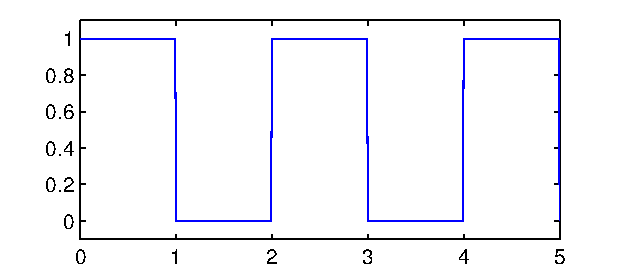
\includegraphics[width=.5\columnwidth]{imgs/fourier/sig_creneau}
        \end{itemize}
      \end{column}
      \begin{column}{6cm}
        \begin{itemize}
        \item $x(t)=\sum_{i=-\infty}^\infty 1_{[iT_0,iT_0+T_0/2 ]}(t)$
        \item $a_0=1, a_k=0 \quad \forall k >0$
        \item $b_k=\frac{2}{\pi k}$ for $k$ odd else $b_k=0$
        \end{itemize}
      \end{column}
    \end{columns}
  \end{exampleblock}

    
 \begin{block}{Complex harmonic decomposition}
    One can express periodic $x(t)$ of period $T_0=\frac{2\pi}{w_0}$ integrable on the period as
  $$
  x(t) = \sum_{k=-\infty}^{^\infty}  c_k  e^{jkw_0t} \quad \quad \text{ avec }
  w_0= \frac{2 \pi }{T_0}
  $$
  where the coefficients $c_k$ are called the  \textbf{complex Fourier coefficients} and can be computed with
  $$
  c_k = \frac{1}{T_0} \int_{T_0} x(t) e^{-j k w_0t}dt = \frac{1}{T_0} \int_{0}^{T_0} x(t) e^{-j k w_0t}dt = \frac{1}{T_0} \int_{-T_0/2}^{T_0/2} x(t) e^{-j k w_0t}dt
  $$
    \end{block}
  \vspace{-5mm}
    \begin{block}{Relations between decompositions}
     Using the Euler formula we can show that $a_k$ and $b_k$ and the $c_k$ coefficients are related by
  $$
  \frac{a_0}{2}= c_0 \quad \quad a_k = c_k + c_{-k} \quad \quad b_k =
  j(c_k - c_{-k})
  $$
  % et
  % $$
  % c_k=\frac{a_k -j b_k}{2} \quad \quad c_{-k}=\frac{a_k +j b_k}{2}
  % $$
  
  Note that if $x(t)$ is an even function then the
  $b_k=0$ , and if $x(t)$ is odd then $a_k=0$.
    \end{block}

  %\lipsum[2-4]
\section{Fourier transform}
\label{sec:fourier-transform}


\subsection{Definition}
\label{sec:}

    The Fourier Transform (FT) of a signal  $x(t)$ can be expressed as
    \index{Fourier Transform}

    \begin{equation}
      \mathcal{F}[x(t)]= X(f) = \int_{-\infty}^\infty e^{- i 2 \pi f t} x(t) d t 
      \label{eq:fourier_tranform}
    \end{equation}
    When it exists the inverse Fourier transform is defined as
    \begin{equation}
      \mathcal{F}^{-1}[X(f)] = x(t)= \int_{-\infty}^\infty e^{  2 i  \pi f t} X(f) d f
      \label{eq:inverse_fourier}
    \end{equation}

    \begin{itemize}
      \item Note that the $\hat \;$ operator is also often used for the Fourier
      transform $\hat x$ of $x$.
      \item In signal processing the references often use $j$ instead of $i$
      for the imaginary number ($i$ is a measure of current).
      % \item The FT relations are denoted in this course as follows:
      % $$
      % x(t) \rightleftharpoons X(f)
      % $$
      \item The FT is a change of representation for the function $x$ from the temporal representation to the harmonic (frequency) representation.
   %   \item Existence of the inverse Fourier transform is complex and discussed later.
    \end{itemize}

    % \begin{align}
    % \label{eq:TFL1}
    % &[\TFA{f}](\xi)= \hat{f}(\xi) = \int_{\rset} \rme^{- \rmi 2 \pi \xi x} f(x) \rmd x \\
    % &[\TFAC{f}](x) = \int_{\rset} \rme^{ \rmi 2 \pi \xi x} \hat{f}(\xi) \rmd x
    % \end{align}
    % On appelle $\TFA{f}$ (not{\'e} aussi $\TF f$) la \emph{Transform{\'e}e de Fourier} de $f$ et $\TFAC{f}$  (not{\'e} aussi $\TFC f$) la
    % transform{\'e}e de Fourier conjugu{\'e}e de $f$.



    $$
    x(t)= \int_{-\infty}^\infty \rme^{ \rmi 2 \pi f t} X(f) \rmd f
  $$

  \begin{block}{Harmonic representation}
    \begin{itemize}
    \item The FT represents the signal in the frequency domain.
    \item $|X(f)| $ is the magnitude of a sinusoidal signal for frequency $f$.
\item $Arg(X(f)$ is the phase of the sinusoidal signal.
    \item For a real signal $x(t)$, $X(f)=X(-f)^*$ and an informal interpretation would be
      \begin{align}
        x(t) &= \int_{-\infty}^{+\infty} X(f) e^{i2\pi f t} df= \int_{-\infty}^{+\infty} |X(f)| e^{i2\pi (f t+Arg(X(f)))} df\\
        &\approx X(0)+2
        \int_{0+}^{+\infty} |X(f)| \cos(2\pi (f t+Arg(X(f))) )\label{eq:1}
      \end{align}
    \item The modulus and argument of the FT allow identification of the frequency content of the signal and its phase.
   % \item This representation allows for simple interpretation of 
    \end{itemize}
  \end{block}


  \paragraph{Fourier Transform in $L_p(\R)$}



  \begin{itemize}
    \item For $1 \leq p \leq 2 $ the FT maps from $L_p(\R)$ to
    $L_q(\R)$ with $\frac{1}{p}+\frac{1}{q}=1$.
    \item Consequence of the Riesz–Thorin theorem.
      \item The TF of an absolute integrable function is bounded (Example : rectangle).
   %   \item The TF of a bounded function is absolute integrable.
   %   \item T
  \end{itemize} \vspace{-3mm}
  
  
  \begin{block}{Parseval-Plancherel identity in $L_2$}
    The TF of an $L_2$ function is $L_2$. Note that  $L_2$ is a Hilbert
      space of inner product:
      $$ <x,y> = \int_{-\infty}^\infty x(t)y^*(t)dt$$
    For two functions $x,y\in L_2(\R)^2$ of respective TF $X,Y\in L_2(\R)^2$  the
    Parseval-Plancherel identity states that
    \begin{equation}
      <x,y> =  \int_{-\infty}^\infty x(t)y^*(t)dt= \int_{-\infty}^\infty X(f)Y^*(f)df
      \label{eq:parseval}
    \end{equation}
\begin{equation}
    <x,x> = \int_{-\infty}^\infty |x(t)|^2dt= \int_{-\infty}^\infty |X(f)|^2df
        \label{eq:parseval2}
\end{equation}
      which means that the energy of a signal is preserved by FT.
  
  
  \end{block}
  
  More details in \cite[Chap. 5.A]{hunter2019notes} and \cite[Chap. 1]{mallat2015traitement}


  \frametitle{Fourier Transform in $\R^d$}

  The Fourier Transform can be naturally extended to functions in $\R^d$.

  \begin{block}{Fourier Tansform in $\R^d$}
    Let $x(\v): \R^d \rightarrow \mathbb{C}$, the Fourier Transform of $x$ can be expressed as 
    \begin{equation}
      \mathcal{F}[x(\v)]= X(\u) = \int_{\R^d} x(\v) e^{-2i\pi <\v,\u>} \rmd \v 
      \label{eq:fourier_tranform_rd}
    \end{equation}
    When it exists the Inverse FT is defined as
    \begin{equation}
      \mathcal{F}^{-1}[ X(\u)]= x(\v) = \int_{\R^d} X(\u) e^{2i\pi <\v,\u>} \rmd \u 
      \label{eq:in_fourier_tranform_rd}
    \end{equation}\vspace{-2mm}
    \begin{itemize}
      \item $\u \in \R^d$ is a directional frequency. 
      \item All the properties of the 1D FT are preserved (duality, convolution, ...)
      \item With $d=2$, frequency representation of black and white images.
      \item With large $d$, approximation for efficient kernel approximation in machine learning \cite{rahimi2008random}.
    \end{itemize}
  \end{block}

  \frametitle{Fourier transform and angular frequency}
  \begin{itemize}
  \item The FT in this course is a function of frequency $f$ (in Hz).
  \item Another common way to represent frequency is the angular frequency $w$ (in rad/s) such that
%  \item Frequency and angular frequency are related with
$$w=2\pi f,\quad \quad\quad f=\frac{w}{2\pi}$$
\item When using angular frequency the FT is non-unitary meaning that :
 $$   \mathcal{\tilde F}[x(t)]= \tilde X(w) = \int_{-\infty}^\infty \rme^{- \rmi w t} x(t) \rmd t  $$
 $$   \mathcal{\tilde F}^{-1}[X(f)] = x(t)= \frac{1}{2\pi}\int_{-\infty}^\infty \rme^{ \rmi w t} \tilde X(w) \rmd w $$
 \item There exists a unitary angular frequency FT that scales both FT and IFT by $\frac{1}{\sqrt{2\pi}}$.
  \item In the following we will sometime use the FT as a function of the angular frequency:
  $$ \tilde X(w)=X\left(\frac{w}{2\pi}\right)$$

 % \item This is a change of variable in the function but not a FT with $w$ !
  \end{itemize}

  \subsection{Examples of Fourier Transform}
  \label{sec:}

  \begin{exampleblock}{Rectangular function}
    %\vspace{5mm}
      \begin{columns}
          \begin{column}%{.5\linewidth}
     \begin{equation}
      \label{eq:echelon}
      \Pi_T(t)=
      \begin{cases}
        1/T& \text{if } |t|< T/2\\
        1/2T& \text{if }  |t|= T/2\\
        0& \text{else}
      \end{cases}
    \end{equation}
    
      The Fourier transform is
      \begin{align*}
        \mathcal{F}[\Pi_T(t)]=&   \frac{1}{T}\int_{-T/2}^{T/2} e^{- i 2 \pi f t} \rmd t \\
        =& \left[\frac{-\rme^{- \rmi 2 \pi f t}}{\rmi 2 \pi fT}\right]_{-T/2}^{T/2}\\
        =&  \frac{\rme^{\rmi \pi f T}-\rme^{- \rmi \pi f T}}{\rmi 2 \pi fT}\\
        =& {\frac{\sin(\pi f T)}{\pi f T} = \text{sinc}(\pi f T)}
      \end{align*} 
    % $$
    % \mathcal{F}[\Pi_T(t)]= \beamer{\frac{\sin(\pi f T)}{\pi f T} = \text{sinc}(\pi f T)}
    % $$
    with 
    $\text{sinc}(t)= \frac{\sin(t)}{t}\quad\text{ and } \text{sinc}(0)=1$

          \end{column}
          \begin{column}%{.4\linewidth}
            \begin{center}
            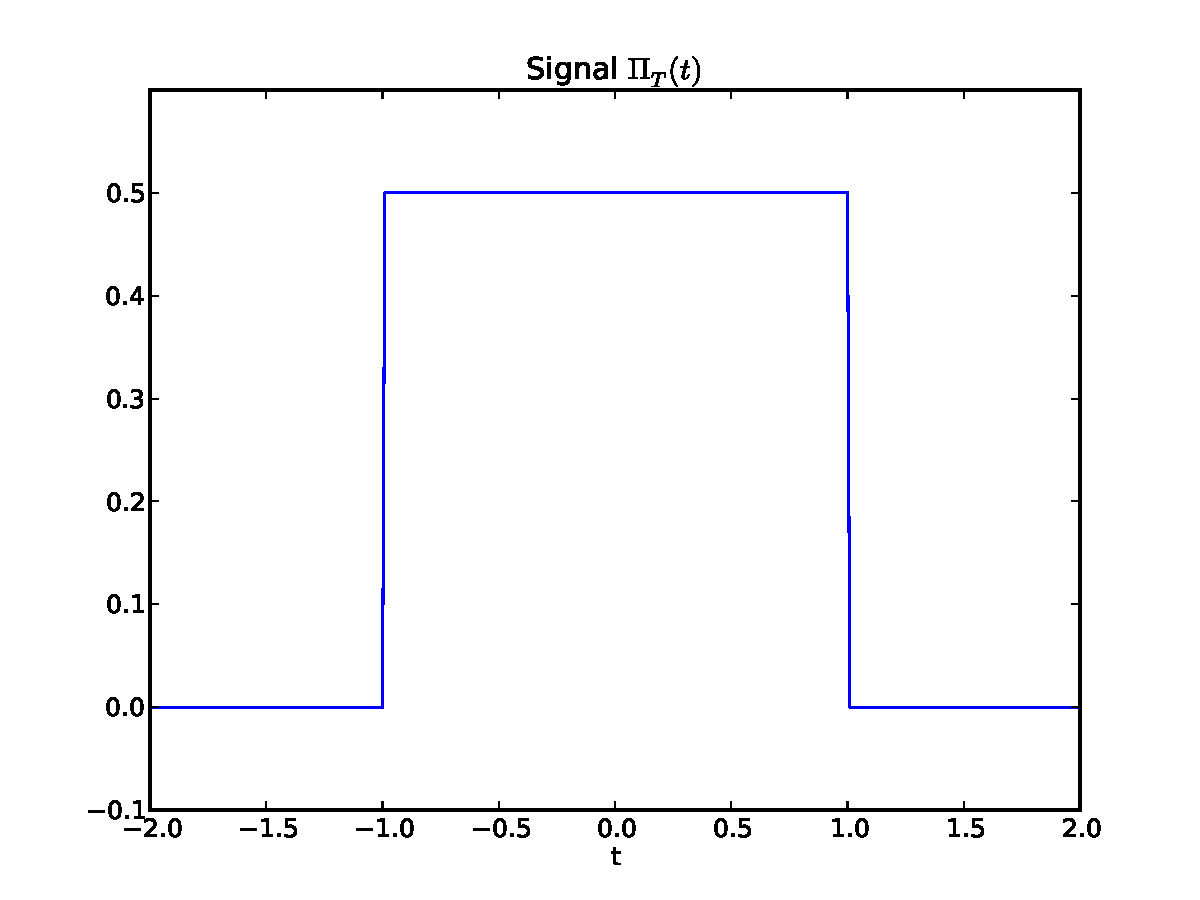
\includegraphics[width=.45\columnwidth]{imgs/fourier/sig_porte_ft.pdf}
            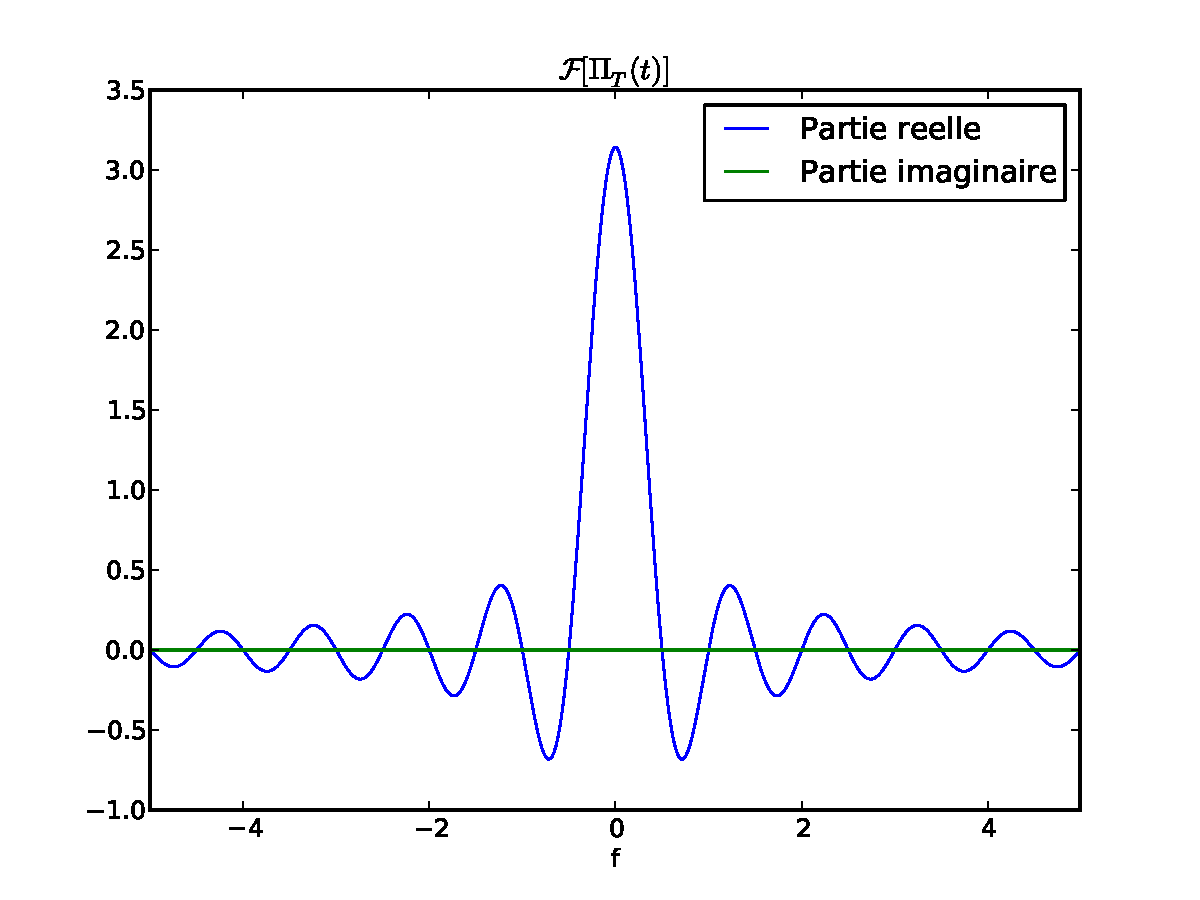
\includegraphics[width=.45\columnwidth]{imgs/fourier/ft_sig_porte_ft.pdf}
          \end{center}
         \end{column}
        \end{columns}
    
    
      \end{exampleblock}


      \begin{exampleblock}{Decreasing exponential}
        \vspace{-5mm}
          \begin{columns}
              \begin{column}%{.5\linewidth}
        $$x(t) = e^{-at} \Gamma(t), \quad   \Gamma(t)=
        \begin{cases}
          1& \text{for } t>0\\
          1/2& \text{for } t=0\\
          0& \text{else}
        \end{cases}$$
        with $a>0$
        
        The Fourier transform is
        \begin{align*}
          \mathcal{F}[e^{-at} \Gamma(t)]=&  \int_{0}^\infty e^{-at} \rme^{- \rmi 2 \pi f t}  dt\\
          =&  \int_{0}^\infty e^{-(a+ \rmi 2 \pi f)t} dt\\
          =& \left[\frac{\rme^{-(a+ \rmi 2 \pi f)t}}{-(a+ \rmi 2 \pi f)}\right]_0^\infty\\
          =&\frac{1}{a+ i 2 \pi f}
        \end{align*}
        % $$
        % X(f)= \beamer{\frac{1}{a+ j 2 \pi f}}
        % $$
               \end{column}
              \begin{column}%{.4\linewidth}
                \begin{center}
                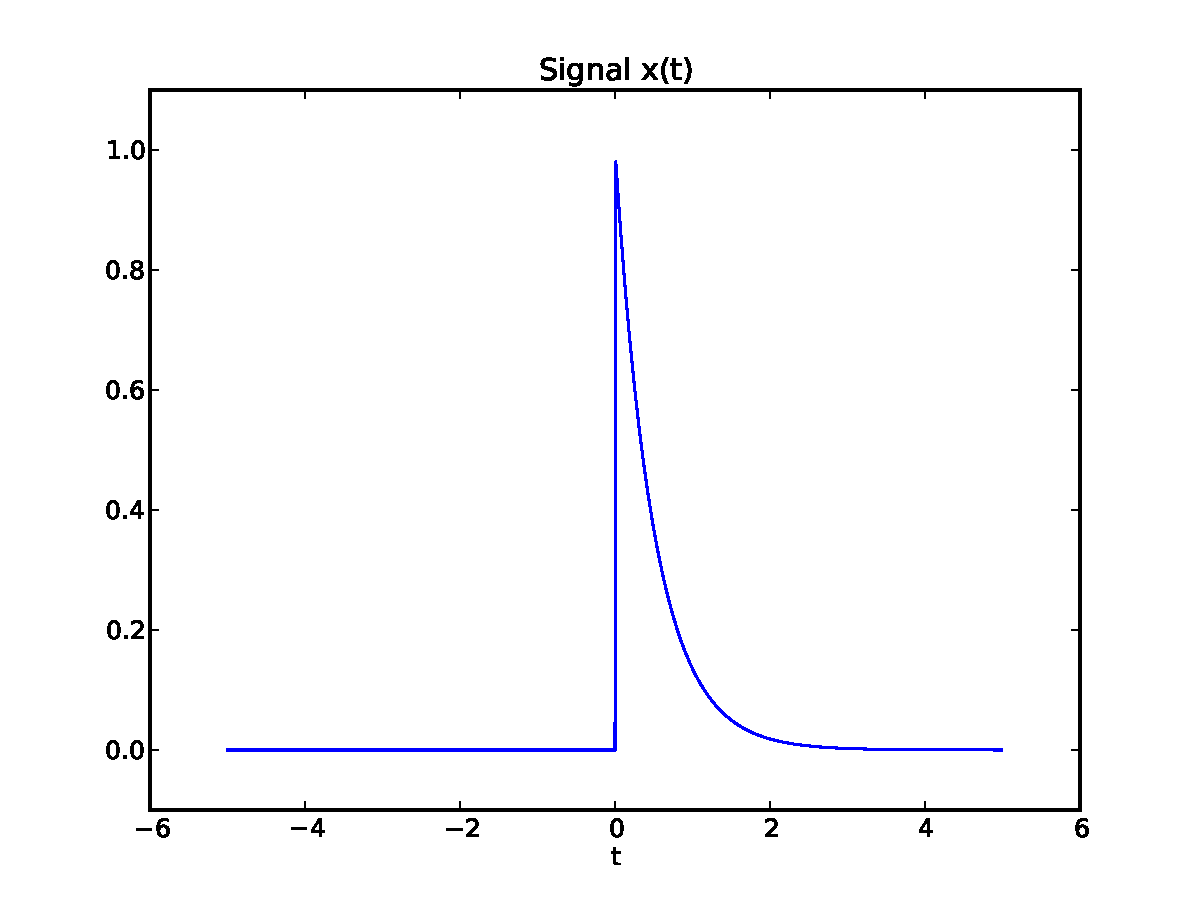
\includegraphics[width=.45\columnwidth]{imgs/fourier/sig_exp_ft.pdf}
                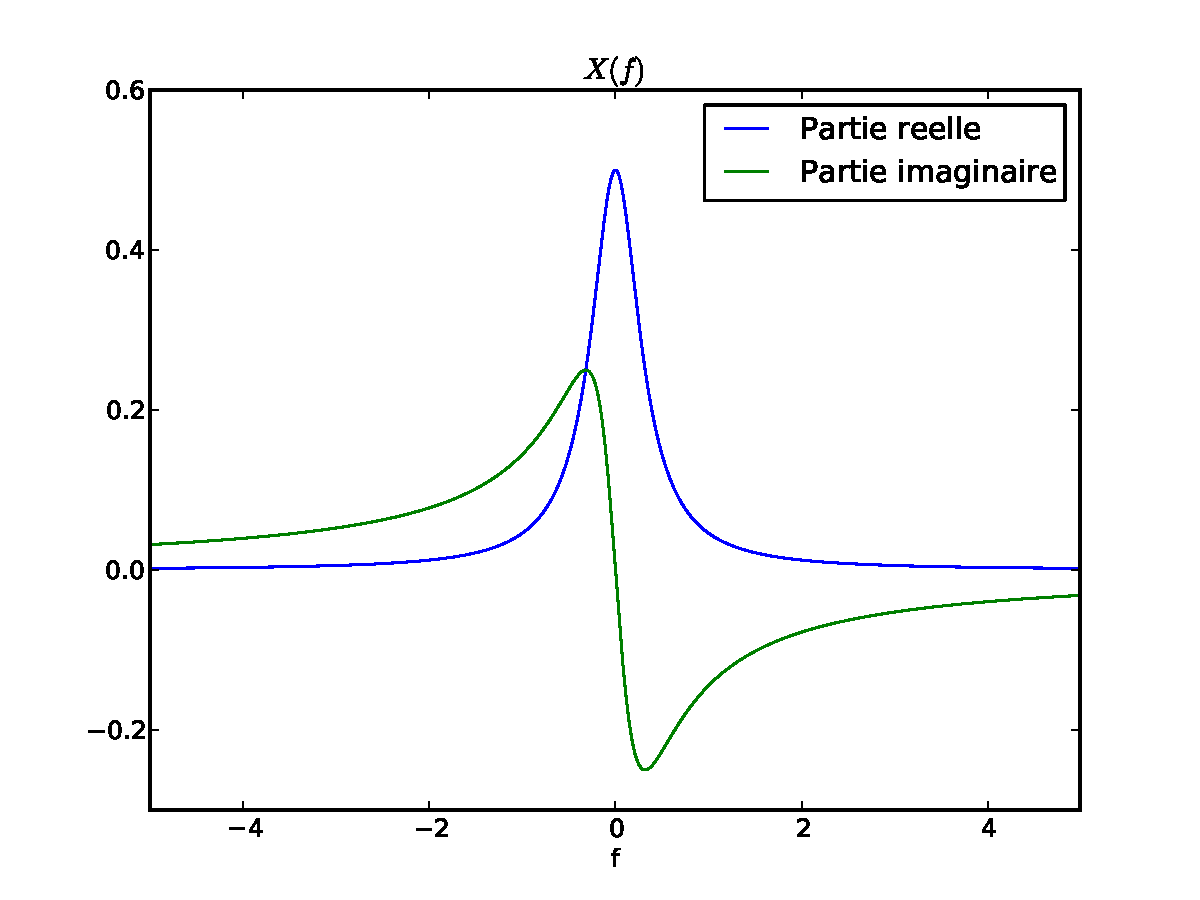
\includegraphics[width=.45\columnwidth]{imgs/fourier/ft_sig_exp_ft.pdf}
              \end{center}
             \end{column}
            \end{columns}
        
          \end{exampleblock}


\subsection{Properties of the Fourier Transform}
\label{sec:}

\begin{block}{Linearity}
    Ley $x_1(t)$ and $x_2(t)$ two signals of TF $X_1(f)$ and $X_2(f)$ respectively. 
  
  For $a \in \R$ and $b \in \R$, we have :
  
  $$
  \mathcal{F}[a x_1(t) + b x_2(t)]=  a X_1(f) + b X_2(f)
  $$
  
  %\begin{demo}
    Comes from the linearity of the integration.
 % \end{demo}
  \end{block}
  
  
  \begin{block}{Time shift}
    Let $x(t)$ be a signal of FT $X(f)$. 
  
  For $t_0 \in \R$, let $x(t-t_0)$ a time shift of  $x(t)$ then we have:
  $$
  \mathcal{F}[x(t-t_0)]= e^{-i 2 \pi t_0f}X(f)
  $$
  %\begin{demo} 
    Change of variable in the integral.
  %\end{demo}
  \end{block}
  

  


  \begin{block}{Frequency shift}

    Let $x(t)$ be a signal of FT $X(f)$ then we have 
  $$
  \mathcal{F}\left[e^{i 2 \pi f_0t} x(t) \right]= X(f-f_0)
  $$
  Multiplication by a complex exponential of frequency $f_0$, translates the TF by
  $f_0$.
  
  %\begin{demo}
     Regroup exponentials in the integral.
  %\end{demo}
\end{block}


\begin{block}{Time scaling}
  Let $x(t)$ be a signal of FT $X(f)$  and $a$ a scaling $a \neq 0$ then we have
$$
\mathcal{F}[x(at)]= \frac{1}{|a|} X\left(\frac{f}{a}\right)
$$
%\begin{demo} 
    Change of variable for separate cases $a>0$ and $a < 0$.
%\end{demo}
\end{block}




\begin{block}{Derivation}
    Let $x(t)$ be a signal of FT $X(f)$ then we have 
  $$
  \mathcal{F}\left[\frac{d x(t)}{ dt }\right]=  j 2 \pi f X(f)
  $$
  % \begin{demo} Dériver le deux termes définissant la
  %   transformée de Fourier par $t$.
  % \end{demo}
  \end{block}
  
  
  \begin{block}{Integration}
    Let $x(t)$ be a signal of FT $X(f)$ such that
    $\int_{-\infty}^\infty x(t) dt = 0$ then we have
  $$
  \mathcal{F}\left[\int_{-\infty}^t x(u) du \right]= \frac{1}{i 2 \pi f }  X(f)
  $$
  If   $\int_{-\infty}^\infty (x(t)-c) dt = 0$ where $c$ is often called the constant term, we have
  $$
  \mathcal{F}\left[\int_{-\infty}^t x(u) du \right]= \frac{1}{i 2 \pi f }  X(f)+ c\delta(f)
  $$
  where $\delta(f)$ is the Dirac delta.
  \end{block}

  Those two properties can be used to solve Ordinary Differential Equations
  (ODE).
  


\begin{block}{Even and odd signals}
    \begin{center}
      \begin{tabular}{|l|l|}
        \hline
        $x(t)$ & $X(f)$\\ \hline
        Even real & Even real \\
        Odd real & Odd imaginary \\
        Even imaginary & Even imaginary\\
        Odd imaginary & Odd real\\ \hline
      \end{tabular}
    
      
    \end{center}
    For a real signal $x(t)$ : $X(f)=X(-f)^*$ 
    \end{block}
      % \begin{itemize}
      % \item Si un signal $x(t)$ est un signal réel et pair alors $X(f)$
      %   est réelle et paire.
    
    
      % \item Si un signal $x(t)$ est un signal réel impair alors $X(f)$ est
      %   imaginaire pure et impaire.
      % \end{itemize}
    
    
    
    \begin{block}{Conjugate signal}
      Let $x(t)$  be a signal of FT $X(f)$ and
      $x^*(t)$ its complex conjugate, then we have
    $$
    \mathcal{F}[x^*(t)] = X^*(-f)
    $$
    \end{block}


    \paragraph{Duality of the Fourier Transform}
    

Let $x(t)$ be a signal of FT $X(f)$. 
% Par définition, on a
% $$
% X(f)= \int_{-\infty}^{+\infty} x(t) e^{-j2 \pi f t} dt 
% $$
% et la définition de la transformée inverse donne
% $$
% x(t)= \int_{-\infty}^{+\infty} X(f) e^{j2 \pi f t} df
% $$
% De par cette dernière définition
When the inverse Fourier transform exists we can write
$$
x(-t)= \int_{-\infty}^{+\infty} X(f) e^{j2 \pi f (-t) } 
df = \int_{-\infty}^{+\infty} X(f) e^{-j2 \pi f t } 
df 
$$

\begin{itemize}
  \item The last term is the TF of function $X(f)$.
  \item This means that if $ \mathcal{F}[x(t)]=X(f)$ then
  $$ \mathcal{F}[X(t)]= x(-f)$$
  \item Applying twice the TF operator to $x(t)$ returns $x(-t)$: 
  \ $ \mathcal{F}[\mathcal{F}[x(t)]]=x(-t)$
\end{itemize}

% Le dernier terme de l'égalité correspond à la transformée
% de Fourier de la fonction $X(f)$. En intervertissant
% les variables temporelles $t$ et les variables
% fréquentielles $f$, on a donc
% si 
% $
% x(t) \rightarrow X(f)
% $ alors

% $$
% X(t) \rightarrow x(-f)$$


%\begin{example}
     For the rectangular function $ \Pi_T(t)$ : 

$$
\begin{array}{l}
  \Pi_T(t) \rightarrow  \text{sinc}(\pi f T) \\
  \text{sinc}(\pi T t )\rightarrow {\Pi_T(-f) =\pause \Pi_T(f)}
\end{array}
$$


\paragraph{Convolution and Fourier Transform}
\begin{block}{Convolution and Fourier Transform}
  Let two signals $x(t)$ and $h(t)$ of respective Fourier transform $X(f)$ and
  $H(f)$ then 
  \begin{equation}
    \mathcal{F}
    [ x(t)\star h(t)]  = X(f)H(f)
    \label{eq:tf_conv}
  \end{equation}\vspace{-5mm}
  \begin{itemize}
    \item The TF of a convolution is a pointwise multiplication in frequency.
    \item The complex exponential function is the eigenvector for the convolution operator.
    \item Easy interpretation of the effect of a linear filtering.

   % \item 
  \end{itemize}
\end{block}

\begin{block}{Proof}
 % Let $y(t)= x(t)*h(t)$. 
  \begin{align*}
    \mathcal{F}
    [ x(t)\star h(t)]&=\int_{-\infty}^\infty \int_{-\infty}^\infty e^{-2i\pi f t} x(u)h(t-u)du dt\\
    &=\int_{-\infty}^\infty \int_{-\infty}^\infty e^{-2i\pi f (u+v)} x(u)h(v)du dv\\
    &= \left\{\int_{-\infty}^\infty  e^{-2i\pi f u} x(u) du\right\}\left\{ \int_{-\infty}^\infty e^{-2i\pi f v} h(v) dv\right\} = X(f)H(f)
  \end{align*}
  with the change of variable $v=t-u$.
\end{block}



\begin{block}{Fourier transform and Dirac delta}
  \begin{itemize}
    \item Fourier Transform of $\delta(t)$ and  $\delta(t-t_0)$:
    $$\mathcal{F}[\delta(t)] = \int_{-\infty}^{+\infty} \delta(t) 
    e^{-i 2\pi f t}dt ={ e^0= 1}$$
 %   \item Fourier Transform  of $\delta(t-t_0)$:
    $$\mathcal{F}[\delta(t-t_0)] = 
    e^{-i 2\pi f t_0} $$   
    \item By duality of FT we have:
    $$ \mathcal{F}[1] =  \delta(t) $$
    $$ \mathcal{F}[e^{i 2\pi f_0 t}] = \delta(f-f_0) $$
    \item Convolution
    $$ \mathcal{F}[x(t)\star \delta(t)] = 1X(f)= X(f)$$
    $$ \mathcal{F}[x(t)\delta(t)] = X(f)*1= \int_{-\infty}^\infty X(f)df=x(0)$$
  \end{itemize}
\end{block}


\frametitle{The dirac comb}

\begin{itemize}
  \item The dirac comb is expressed as
  \begin{equation}
    \Sh_T(t)=\sum_{k=-\infty}^\infty \delta(t-kT)
    \label{eq:dirac_comb}
  \end{equation}
  where $\Sh$ is the Cyrilic Sha symbol.
  \item The Fourier Transform of the dirac comb is 
  \begin{equation}
    \mathcal{F}[\Sh_T(t)]=\sum_{k=-\infty}^\infty e^{2i\pi k T f}= \frac{1}{T}\sum_{k=-\infty}^\infty \delta\left(f-\frac{k}{T}\right) =  \frac{1}{T}\Sh_{\frac{1}{T}}(f)
    \label{eq:ft_dirac_comb}
  \end{equation}
  where the second equality comes from the Poisson summation formula.
  \item The dirac comb is used to perform a regular temporal sampling.
  \item Multiplying a signal by the dirac comb corresponds to a convolution by a dirac comb in the Frequency domain (and vice versa).
\end{itemize}
%\end{example}


\frametitle{Fourier transform of periodic signals}


\begin{block}{Cosine}
$$
x(t)= \cos(2 \pi f_0 t) \quad \quad \text{with } f_0 > 0
$$
  \begin{itemize}
  \item Bounded signal with unbounded energy.
  \item Intuitively this signal contains only one frequency ($f_0$)
  \item Its TF can be computed thanks to the dirac distribution.
  \end{itemize}
\end{block}
\begin{block}{FT of trigonometric functions}
  $$
\mathcal{F}\left[\cos(2 \pi f_0 t) = \frac{e^{j2\pi f_0t} + e^{-j2\pi f_0t} }{2}\right]
= %\pause
\frac{1}{2}\delta(f-f_0) + \frac{1}{2}\delta(f+f_0) 
$$
$$
\mathcal{F}\left[\sin(2 \pi f_0 t) = \frac{e^{j2\pi f_0t} - e^{-j2\pi f_0t} }{2i}\right]
= %\pause
\frac{1}{2i}\delta(f-f_0) - \frac{1}{2i}\delta(f+f_0) 
$$
The FT of sine and cosine is equal to $0$ everywhere except on the frequency $f_0$ of the functions.
\end{block}




\begin{block}{Fourier transform of periodic signal}
    Let $x(t)$ be a periodic signal of period $T_0$, it can be expressed as the following complex Fourier series:
    $$x(t)= \sum_k c_k e^{i 2 \pi \frac{k}{T_0}t} $$
    Its Fourier transform can be expressed as 
    $$
  X(f)=\mathcal{F}[x(t)]= %\pause 
  \sum_k c_k \delta\left(f-\frac{k}{T_0}\right)
    $$
    \begin{itemize}
      \item The FT of a periodic signal of period is null except on frequencies $\frac{k}{T_0},\;k\in\mathbb{N}$.
      \item $\frac{1}{T_0}$ is the fundamental frequency, $\frac{k}{T_0}$ with $|k|\geq 2$ are called the harmonics.
      \item The TF of a periodic function is a weighted sum of diracs.
      \end{itemize}
  \end{block}


  \frametitle{How to compute a Fourier Transform ?}

  \begin{block}{Usual steps}
    \begin{enumerate}
      \item Use known FT pairs if possible.
      \item Express the function as a composition of operations with known properties:
        \begin{itemize}
          \item Linearity, time shift
          \item Convolution
          \item Duality
        \end{itemize}
      \item Use the properties of FT on the composition.
      \item Check properties (FT of even/odd function) to detect easy mistakes.
    \end{enumerate}
    As a rule : try to avoid computing the integral but sometime you have to do it.
  \end{block}

   

%\lipsum[2-4]
\section{Frequency response and filtering}
\label{sec:freq-response}

\subsection{Frequency response of an LTI system}
\label{sec:}

\begin{block}{Impulse response and frequency response}
    \begin{itemize}
      \item Most LTI systems can be expressed as a convolution of the form:
     $$y(t)=x(t)\star h(t)$$
     where $h(t)$ is called the impulse response (the response of the system to an input $x(t)=\delta(t)$)
     \item The Fourier transform of the LTI system relation is
     \begin{equation}
      \label{eq:rep_freq_syst}
      Y(f)=H(f)X(f)
    \end{equation}
    \item The frequency response $H(f)$ (also called transfer function) of the LTI system is the Fourier transform of $h(t)$:
    \begin{equation}
      \label{eq:rep_freq_syst2}
      H(f)=\frac{Y(f)}{X(f)}
    \end{equation}
    \end{itemize}

  \end{block}


  \begin{block}{Response to a mono-frequency signal}
    \begin{itemize}
    \item For a system of impulse response $h(t)$ with an input $x(t)=e^{2j\pi f_0 t}$
   % \item Signal en entrée de la forme $x(t)=e^{2j\pi f_0 t}$.
  %  \item Signal de sortie:\pause
\begin{align*}
  y(t) &= \int_{-\infty}^{+\infty}h(\tau)e^{2j\pi f_0 h(t-\tau)}d\tau\\
&= e^{2j\pi f_0 t} \int_{-\infty}^{+\infty}h(\tau)e^{- 2 j\pi f_0
  h\tau}d\tau\\
&=e^{2j\pi f_0 t} H(f_0)=x(t)H(f_0)
\end{align*}
\item An input signal with unique frequency $f_0$ is multiplied by $H(f_0)$.
\item Its amplitude is multiplied by $|H(f_0)|$ and a phase $Arg(H(f_0))$ is added.
\item The complex exponential is an eigenvector of the convolution operator.
    \end{itemize}

  \end{block}

\begin{block}{Static gain}
  The complex static gain is the constant $K$ such that
  % $$K=H(0)$$ 
  % It can be obtained from the impulse response as:
  \begin{equation*}
    K=H(0)=\int_{-\infty}^{+\infty}h(t)dt
  \end{equation*}
\end{block}



\begin{block}{Ordinary Differential Equation (ODE)}
    The system is defined by an equation of the form:
    \begin{equation}
      \label{eq:edo2}
      a_0y(t)+a_1\frac{dy(t)}{dt}+\dots+a_n\frac{d^ny(t)}{dt^n}=
      b_0x(t)+b_1\frac{dx(t)}{dt} +\dots+b_m\frac{d^mx(t)}{dt^m}
    \end{equation}
    
    % \begin{itemize}
    % \item ODE based system with linear relations are an important class of LTI systems.
    
    % %\item $\max(m,n)$ est l'ordre du système.
    % %\item Également appelées équations différentielles linéaires à coefficients
    % %constants.
    % \item $n$ is the number of derivatives for $y(t)$ and $m$ for $x(t)$.
    % \item The output of the system can be computed from he input by solving Eq.
    %   \eqref{eq:edo}
    % \end{itemize}
    
    \end{block}
    
    \begin{block}{Frequency response of an ODE}
      \begin{itemize}
        \item We recall the properties of the FT for th n-th derivative of a function:
         $$ \mathcal{F}\left[\frac{d^{(n)}x(t)}{dt^n}\right]=(2i\pi
        f)^nX(f)=(iw)^nX(w)$$
        \item The Frequency response of the ODE can be expressed as 
        \begin{equation}
          \label{eq:edo_transf}
          H(w)=\frac{Y(w)}{X(w)}=\frac{b_0+b_1jw+\dots+b_m(jw)^m}{a_0+a_1jw+\dots+a_n(jw)^n}
        \end{equation}
      \end{itemize}
    \end{block}

    
    \subsection{Representation of the frequency response}
    \begin{block}{Frequency interpretation of the frequency response}
      \begin{itemize}
      \item The frequency response of a system gives information on the transformations due to the system.
      \item Quantities that can be plotted :
  \begin{align*}
   % \label{eq:hwcomplex}
    \tilde H(w)&= Re(\tilde H(w))+jIm(\tilde H(w))\\
  &=|\tilde H(w)|e^{jArg(\tilde H(w))}
  \end{align*}
  %avec $Arg(w)=\tan^{-1}(\frac{Im(H(w)}{Re(H(w)})$
  \vspace{-5mm}
  \begin{itemize}
  \item $|\tilde H(w)|$ modulus of the frequency response.
  \item $Arg(\tilde H(w))=\angle
  \tilde H(w)=\tan^{-1}\left(\frac{Im(\tilde H(w)}{Re(\tilde H(w)}\right)$ phase in radian.
  \end{itemize}
  
      \end{itemize}
    \end{block}
    \begin{exampleblock}{Graphical representation of systems}
      \begin{itemize}
      \item Bode plot (Modulus+Argument).
      \item Nichols/Black plot (Modulus VS Argument).
      \item Nyquist plot (Real VS Imaginary)
      \end{itemize}
    \end{exampleblock}



    \frametitle{Bode plot}

    \begin{center}
      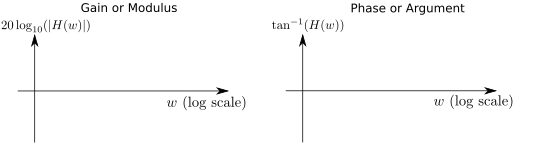
\includegraphics[width=\linewidth]{imgs/fourier/diagramme_bode}
    \end{center}
    
    \begin{block}{Definition}
      The Bode plot of a system is composed of two plots that are function of $w$:
      \begin{itemize}
        \item Magnitude (or gain) in decibels (dB)
        $$\tilde G(w)=20\log_{10}{(|\tilde H(w)|)}$$
        \item Phase in degrees or radians
        $$\tilde \Phi(w)=Arg(H(w)|)=\angle |\tilde H(w)|$$
      \end{itemize}
      The scale of the radial frequency $w$ is logarithmic, which means that for a rational frequency response $H$ one will be mostly piecewise linear.
    \end{block}
    
    \frametitle{Properties of the Bode plot}
    The logarithm and the argument allows for simple diagrams for combination of systems 
    \begin{block}{Multiplication}
      If two LTIs $\tilde H_1(w)$ and $\tilde H_2(w)$ are in series the  the equivalent system is  $\tilde H(w)=\tilde H_1(w)\tilde H_2(w)$ %\pause
      \begin{itemize}
      \item $\tilde G(w)=\tilde G_1(w)+\tilde G_2(w)$
      \item  $\tilde \Phi(w)=\tilde \Phi_1(w)+\tilde \Phi_2(w)$
      \end{itemize}
  
    \end{block}
    \begin{block}{Division}
      If and LTI can be expressed as
   $\displaystyle \tilde H(w)=\frac{\tilde H_1(w)}{\tilde H_2(w)}$
  then%\pause
      \begin{itemize}
      \item $\tilde G(w)=\tilde G_1(w)-\tilde G_2(w)$
      \item  $\tilde \Phi(w)=\tilde \Phi_1(w)-\tilde \Phi_2(w)$
      \end{itemize}
      This is particularly useful for rational frequency responses such as ODE.
    \end{block}

    \begin{center}
        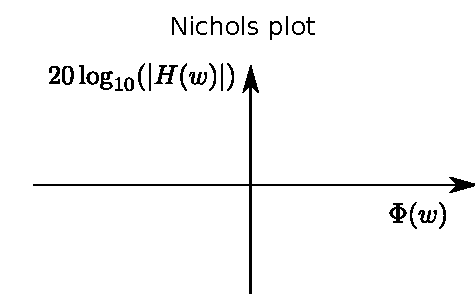
\includegraphics[width=.5\linewidth]{imgs/fourier/diagramme_nichols}
      \end{center}
        \begin{block}{Nichosl plot}
          The Nichols plot (Diagramme de Black in France) is a parametric plot of  $\tilde H(w)$ with 
      $20\log_{10}|\tilde H(w)|$ on y-axis and phase $\tilde \Phi(w)$ on x-axis.
      \begin{itemize}
      \item Show theM odulus/Phase trajectory as a function of $w$.
      \item Can be ploted following the Bode plot $w$.
      \end{itemize}
        \end{block}


        \frametitle{Nyquist plot}
        \begin{center}
          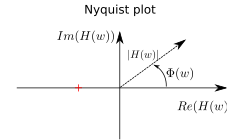
\includegraphics[width=.5\linewidth]{imgs/fourier/diagramme_nyquist}
        \end{center}
        \begin{block}{Definition}
          The Nyquist plot is a parametric plot of  $\tilde H(w)$ with 
        $Real(\tilde H(w))$ on x-axis and  $Imag(\tilde \Phi(w))$ on y-axis.
        \begin{itemize}
          \item Show the trajectory of $\tilde H$ in the complex plane.
          \item Used in system control to study the stability of systems.
        \end{itemize}
        \end{block}


        \frametitle{Frequency response of electronic systems}
 
\begin{block}{Principle}
  Ohm's law can be extended to capacitors and inductors using what is called complex called electrical impedance.
\end{block}
The linear system $i(t)\rightarrow u(t)$ is expressed as
$$\tilde U(w)=\tilde H(w)\tilde I(w)=\tilde Z(w)\tilde I(w)$$
\vspace{-5mm}
\begin{columns}[t]
  \begin{column}%{3cm}
    \begin{block}{Resistor}
      \begin{itemize}
      \item
$u(t)=Ri(t)$
\item \pause $\tilde U(w)=R\tilde I(w)$
\item $Z_R=R$
      \end{itemize}
    \end{block}
  \end{column}
  \begin{column}%{4cm}
    \begin{block}{Capacitor}
      \begin{itemize}
      \item
$u(t)=\frac{1}{C}\int_{-\infty}^ti(u)du$
\item \pause $\tilde U(w)=\frac{1}{jCw}\tilde I(w)$
%\item $U(w)=jLwI(w)$
\item $Z_C=\frac{1}{jCw}$
      \end{itemize}
    \end{block}
  \end{column}
  \begin{column}%{3.5cm}
    \begin{block}{Inductor}
      \begin{itemize}
      \item
$u(t)=L\frac{di(t)}{dt}$
\item \pause $\tilde U(w)=jLw\tilde I(w)$
\item $Z_L=jLw$
      \end{itemize}
    \end{block}
  \end{column}
\end{columns}
The frequency response of passive electronic systems can be computed with simple
computation of complex numbers.

\paragraph{First order system}

\begin{columns}
    \begin{column}%{6cm}
   \begin{itemize}
  \item System
\begin{align*}
x(t)&=Ri(t)+y(t)\\
y(t)&=\frac{1}{C}\int_{-\infty}^ti(v)dv \\
x(t)&=RCy'(t)+y(t)
\end{align*}
  \end{itemize}       
    \end{column}
    \begin{column}%{5cm}
      \begin{center}
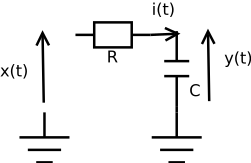
\includegraphics[width=.4\columnwidth]{imgs/fourier/RC2}
\end{center}
    \end{column}
  \end{columns}
  \begin{itemize}
  \item Frequency response\pause
$$ \tilde H(f)=\frac{Y(f)}{X(f)}={\frac{1}{1+RC2j\pi f}}$$
\item Using complex impedance\pause
\begin{equation*}
    \tilde Y(w)=Z_c \tilde I(w) \quad \text{ and } \quad \tilde X(w)= {(Z_R+Z_C) \tilde I(w)}
\end{equation*}
\begin{equation*}
    \tilde H(w)=\frac{ \tilde Y(w)}{\tilde \tilde X(w)}={\frac{Z_c}{Z_C+Z_R}=\frac{1}{1+\frac{Z_R}{Z_C}}=\frac{1}{1+RCjw}}
\end{equation*}
  \end{itemize}

  \begin{block}{Normalized system}
    We reformulate the frequency response as :
\begin{equation}
\label{eq:fobnctransfert_w0}
\tilde H(w)=\frac{1}{1+j\frac{w}{w_0}}
\end{equation}
where $w_0=\frac{1}{\tau}=\frac{1}{RC}$. 
  \end{block}
\textbf{Bode plot}
%\vspace{-5mm}
%\begin{columns}[t]
%\small
%    \begin{column}{6cm}
    \begin{block}{Modulus}\pause
\begin{enumerate}
\item $\tilde H(w)={\frac{1}{1+j\frac{w}{w_0}}}$
\item  $|\tilde H(w)|={\frac{1}{\sqrt{1+\frac{w^2}{w_0^2}}}}$
\item  $\tilde G(w)={20\log_{10}(|H(w)|)=-10\log_{10}(1+\frac{w^2}{w_0^2})}$
\item $\lim_{w\rightarrow 0}
\tilde G(w)={0}$
\item 
$\lim_{w\rightarrow\infty} \tilde G(w)={-10\log_{10}(\frac{w^2}{w_0^2})=-20\log_{10}(w)+20\log_{10}(w_0)}$
\item When $w=w_0$, $\tilde G(w)={-10\log_{10}(2)=-3dB}$
\end{enumerate}
    \end{block}

    \begin{block}{Argument}%\pause
        \begin{enumerate}
        \item $\tilde H(w)={\frac{1}{1+j\frac{w}{w_0}}}$
        \item $\tilde \Phi(w)={\arg(H(w))=-arg(1+jw)=-tan^{-1}(w)}$
        \item  $\lim_{w\rightarrow 0}
        \tilde  \Phi(w)={0}$
        \item   $\lim_{w\rightarrow\infty}\tilde \Phi(w)={-\pi/2}$
        \item  When $w=w_0$, $\tilde \Phi(w)={-tan^{-1}(1)=-\pi/4 \ (-45^\circ)}$
        
        when  $w=10w_0$,
          $\tilde \Phi(w)={-84^\circ}$
        
        when $w=.1w_0$
          $\tilde \Phi(w)={-6^\circ}$
        \end{enumerate}
              \end{block}

                \begin{block}{Bode plot}
                  \begin{center}
                    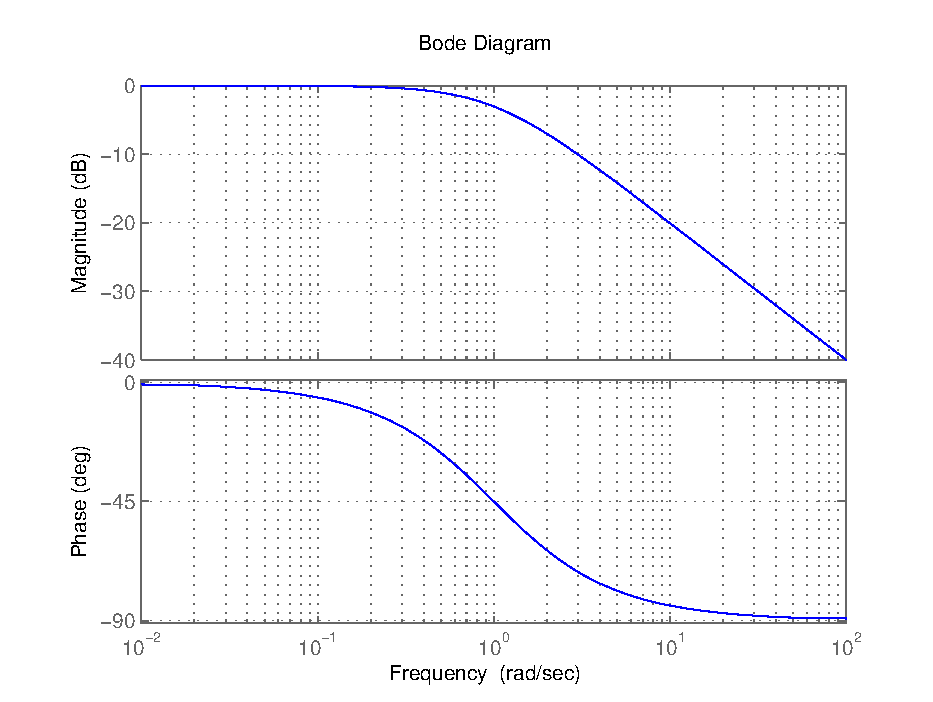
\includegraphics[width=.8\linewidth]{imgs/fourier/bode_rc}
                  \end{center}
                \end{block}

            

                    \begin{block}{Nichols plot}
                  \begin{center}
                    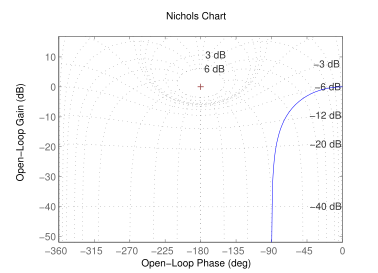
\includegraphics[width=.8\linewidth]{imgs/fourier/nichols_rc}
                  \end{center}
                \end{block}

            

                    \begin{block}{Nyquist plot}
                  \begin{center}
                    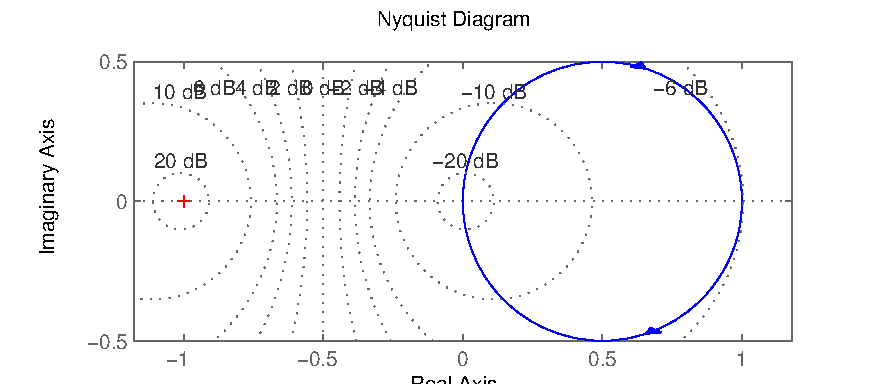
\includegraphics[width=.8\linewidth]{imgs/fourier/nyquist_rc}
                  \end{center}
                \end{block}

\paragraph{Secon order system}

\begin{columns}
    \begin{column}{6cm}
   \begin{itemize}
  \item Complex Impedance
\begin{align*}
\tilde Y(w)&=Z_c\tilde  I(w)\\
\tilde X(w)&= (Z_L+Z_R+Z_C) \tilde I(w)\\
\end{align*}
  \end{itemize}       
    \end{column}
    \begin{column}{5cm}
      \begin{center}
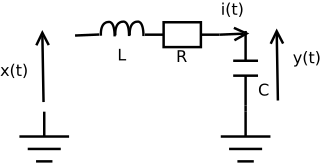
\includegraphics[width=.3\columnwidth]{imgs/fourier/RLC}
\end{center}
    \end{column}
  \end{columns}
  \begin{itemize}
  \item Frequency response
$$ \tilde H(w)=\frac{\tilde Y(w)}{\tilde X(w)}=\pause\frac{Z_C}{Z_L+Z_R+Z_C}=\frac{\frac{1}{jCw}}{\frac{1}{jCw}+R+jLw}$$
\item Normalized frequency response
\begin{equation*}
  \tilde H(w)=\frac{1}{1+RCjw+LC(jw)^2}=\frac{k}{1+2z\frac{jw}{w_n}+(\frac{jw}{w_n})^2}
\end{equation*}%\pause
\begin{itemize}
\item $k$ Static gain : $k=\pause{1}$
\item $z$ damping ratio of the system : $z=\pause {\frac{R}{2}\sqrt{\frac{C}{L}}}$
\item $w_n$ natural frequency of the system : $w_n=\pause {\frac{1}{\sqrt{LC}}}$
\end{itemize}
  \end{itemize}


  \begin{block}{Linear differential equation}
    The second order differential equation corresponding to the system is
        \begin{equation}
      \label{eq:syst_second_ordre}
      \frac{d^2y(t)}{dt^2}+2zw_n \frac{dy(t)}{dt}+w_n^2y(t)=kw_n^2x(t)
    \end{equation}
      \end{block}
      \begin{block}{Factorization}
    The second order system can be factorized as%\pause
    \begin{equation}
      \label{eq:transfsecondordre3}
      \tilde H(w)=\frac{kw_n^2}{(jw-c_1)(jw-c_2)}
    \end{equation}
    with
    
    \begin{align}
      \label{eq:6}
      c_1&={-zw_n+w_n\sqrt{z^2-1}}\\
      c_2&={-zw_n-w_n\sqrt{z^2-1}}
    \end{align}
     $c_1$ and $c_2$ are called the poles of the transfer function.
      \end{block}


      \begin{block}{Response of the system for  $z>1$}
        \begin{itemize}
        \item 
          $c_1$ and $c_2$ are real coefficients.
        \item The FT can be expressed as
          \begin{equation}
            \label{eq:transfsecondordre5}
            \tilde  H(w)=\frac{M}{jw-c_1}-\frac{M}{jw-c_2}
          \end{equation}
          with $M=\frac{w_n}{2\sqrt{z^2-1}}$,
        \item The impulse response of the system is
          \begin{equation*}
            h(t)=M(e^{c_1t}-e^{c_2t})\Gamma(t)
          \end{equation*}
    
        \item The step response of the system is
          \begin{equation*}
            e(t)=\left(1+M\left(\frac{e^{c_1t}}{c_1}-\frac{e^{c_2t}}{c_2}\right)\right)\Gamma(t)
          \end{equation*}
        \end{itemize}
    
      \end{block}


      \begin{block}{Response of the system for $z=1$}
        The FT becomes:
    \begin{equation}
      \label{eq:transfsecondordre3}
      \tilde H(w)=\frac{kw_n^2}{(jw+w_n)^2}
    \end{equation}
    that is the square of one first order system.
    
     The impulse response fo the system can be expressed as
    \begin{equation*}
      h(t)=w_n^2te^{-w_nt}\Gamma(t)
    \end{equation*}
    The step response can be expressed as
    \begin{equation*}
      e(t)=(1-e^{-w_nt}-w_nte^{-w_nt})\Gamma(t)
    \end{equation*}
      \end{block}


      \begin{block}{Response of the system for $z<1$}
        \begin{itemize}
        \item In this case the damping is weak and oscillations appear.
    \item This comes from teh fact that when
     $z<1$ coefficients $c_1$
     and $c_2$ are complex. The impulse response is
    \begin{equation*}
      h(t)=M(e^{c_1t}-e^{c_2t})\Gamma(t)
    \end{equation*}
    \item The step response is
    \begin{equation*}
      h(t)=\frac{w_ne^{-zw_nt}}{\sqrt{1-z^2}}\sin\left(w_nt\sqrt{1-z^2}\right)\Gamma(t)
    \end{equation*}
    that is  a sine with an exponentially decreasing magnitude. 
        \end{itemize}
     
    
    
    
      \end{block}


      \begin{block}{Impulse and step responses}
        \begin{center}
          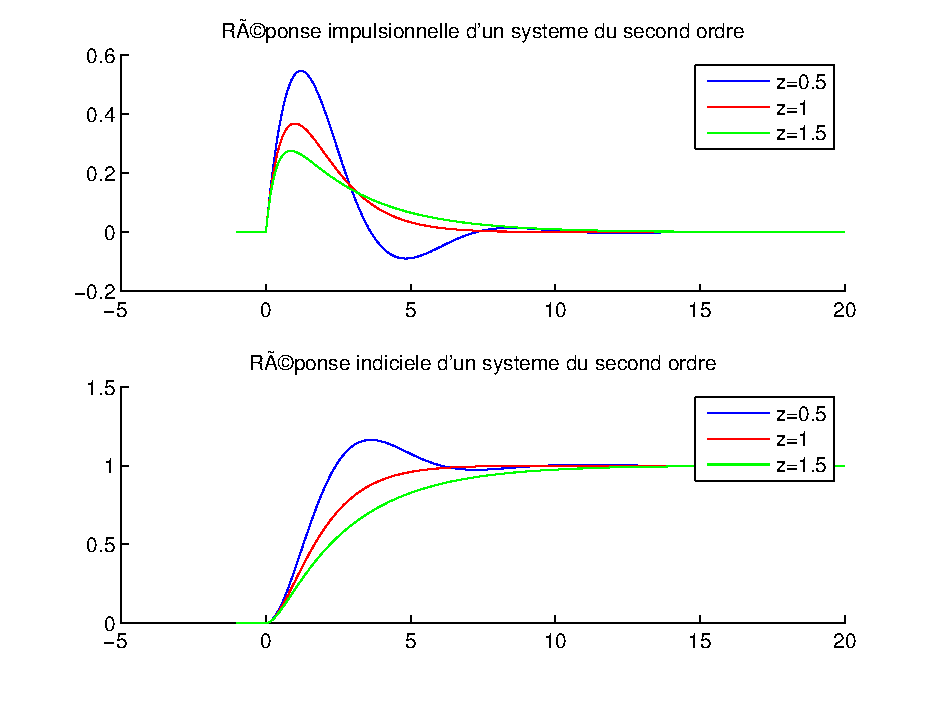
\includegraphics[width=10cm]{imgs/fourier/rep_2o}
        \end{center}
      \end{block}


      \begin{block}{Bode plot}
        We can plot the Bode plot using the normalized frequency response:
    \begin{equation}
      \label{eq:transfsecondordre2}
      H(w)=\frac{k}{\left(\frac{jw}{w_n}\right)^2+2z\left(\frac{jw}{w_n}\right)+1}
    \end{equation}
    \vspace{-5mm}
    \begin{block}{Modulus}
    \pause
    \small
      \begin{enumerate}
    \item $ \tilde  H(w)=\frac{k}{\left(\frac{jw}{w_n}\right)^2+2z\left(\frac{jw}{w_n}\right)+1}$.
    \item  $|\tilde H(w)|=\frac{k}{\sqrt{\left(1-\left(\frac{w}{w_n}\right)^2\right)^2+4z^2\left(\frac{w}{w_n}\right)^2}}$.
    \item  $\tilde G(w)=20\log_{10}(|\tilde H(w)|)=-10\log_{10}\left(\left(1-\left(\frac{w}{w_n}\right)^2\right)^2+4z^2\left(\frac{w}{w_n}\right)^2\right)+20log(k)$
    \item $\lim_{w\rightarrow 0}
    \tilde  G(w)=20log(k)$
    \item 
      $\lim_{w\rightarrow\infty} \tilde G(w)=-10\log_{10}(\frac{w^4}{w_n^4})=-40\log_{10}(w)+40\log_{10}(w_n)$
    \item En $w=w_0$, $\tilde G(w)=-20\log_{10}(2z)+20\log(k)$.
    \end{enumerate}
    \end{block}
      \end{block}

      \begin{block}{Properties of the modulus}
        \begin{itemize}
        \item The modulus of the frequency response for  $z<\sqrt(2)/2$ has a maximum at the following frequency
    \begin{equation*}
      w_{max}=w_n\sqrt{1-2z^2}
    \end{equation*}
    \item The value of the modulus at this frequency is
    \begin{equation*}
      |\tilde H(w_{max})|=\frac{k}{2z\sqrt{1-z^2}}
    \end{equation*}
    
    \item The cutoff frequency at -3dB is equal to
    \begin{equation*}
      w_{-3}=w_n\sqrt{1+2z^2+\sqrt{2-4z^2+4z^4}}
    \end{equation*}
    \end{itemize}
    
      \end{block}

      \textbf{Bode plot}
  \begin{block}{Argument}
\pause
\begin{enumerate}
\item $\tilde H(w)= \frac{k}{\left(\frac{jw}{w_n}\right)^2+2z\left(\frac{jw}{w_n}\right)+1}$.
\item $\tilde \Phi(w)=\arg(H(w))=-arg(\left(\frac{jw}{w_n}\right)^2+2z\left(\frac{jw}{w_n}\right)+1)=-tan^{-1}\left(\frac{2z\frac{w}{w_n}}{1-\frac{w^2}{w_n^2}}\right)$.
\item  $\lim_{w\rightarrow 0}
\tilde  \Phi(w)=0$
\item   $\lim_{w\rightarrow\infty}\tilde \Phi(w)=-\pi(-180^\circ )$
\item  En $w=w_0$, $\tilde \Phi(w)=-tan^{-1}(1)=-90^\circ$, 
\end{enumerate}

  \end{block}

  \begin{block}{Bode plot}
    \begin{center}
      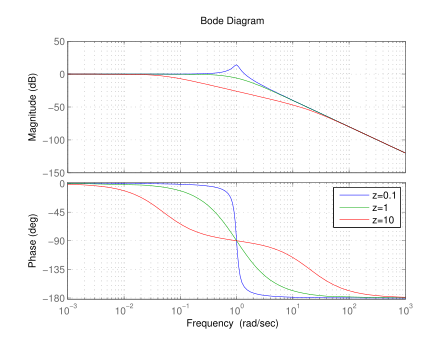
\includegraphics[width=.8\linewidth]{imgs/fourier/bode_2o}
    \end{center}
  \end{block}

  \begin{block}{Nichols plot}
    \begin{center}
      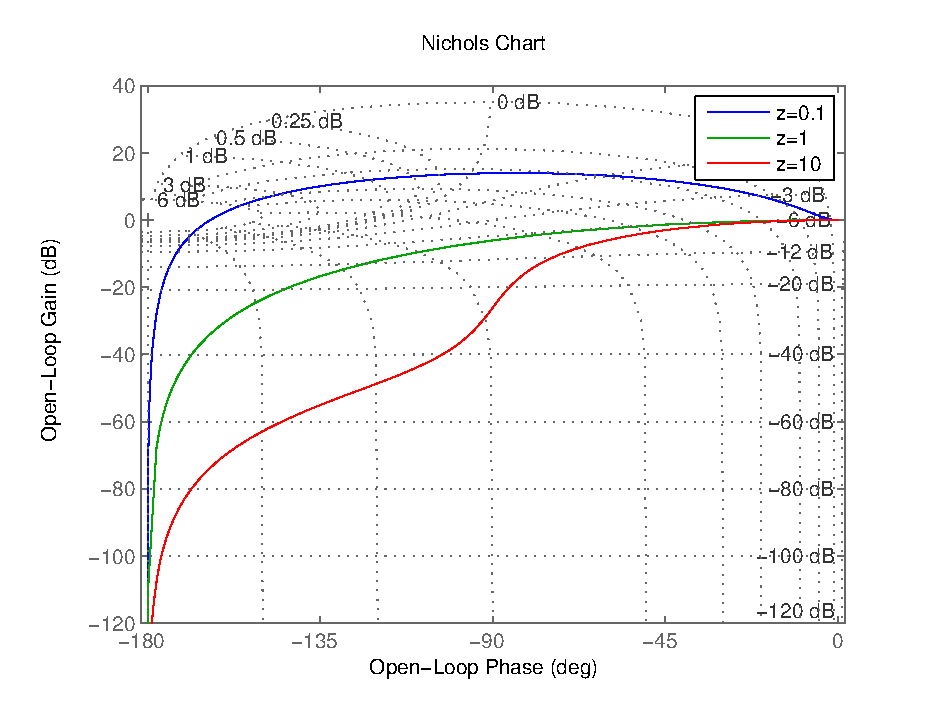
\includegraphics[width=.8\linewidth]{imgs/fourier/nichols_2o}
    \end{center}
  \end{block}

  \begin{block}{Nyquist plot}
    \begin{center}
      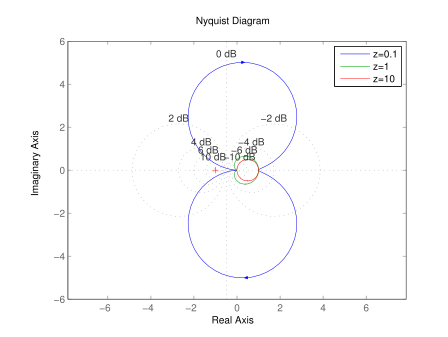
\includegraphics[width=.8\linewidth]{imgs/fourier/nyquist_2o}
    \end{center}
  \end{block}

%\lipsum[2-4]
\section{Applications of analog signal processing}
\label{sec:appli-ft}
%\lipsum[2-4]

\begin{block}{Applications of analog signal processing} \vspace{-1mm}
    \begin{itemize}
        \item Analog signal filtering. 
        \begin{itemize}
            \item Electronic passive and active filters.
            \item Modeling and filtering with physical systems.
        \end{itemize}
        \item Telecommunications. \vspace{-1mm}
            \begin{itemize}
                \item Amplitude modulation.
                \item Multiplexing.
            \end{itemize}
        \item Fourier opticsL\vspace{-1mm}
        \begin{itemize}
            \item Light propagation in perfect lens/mirror systems.
            \item Point spread functions of telescope and cameras.
        \end{itemize}
    \end{itemize}
\end{block}

\subsection{Analog filtering}
\label{sec:analogfiltering}

\begin{block}{Definition}
    Signal processing system that aim at selecting part of the signal and attenuating another part (noise).

Analog filtering as opposed to digital filtering (next course)
  \end{block}


  \begin{block}{Objectives}
    \begin{itemize}
    \item Find a system that transform a signal $x(t)$ to extract pertinent information.
    \item Attenuate noise in a  signal.
    \item Separate several components of a signal (when different frequency bands).
    \end{itemize}
  \end{block}

  \frametitle{Filtering and bandwidth}

  \begin{block}{Gain and Attenuation}

    \begin{itemize}
    \item In order to characterize a filter one uses its 
    Gain/Phase (Bode plot).
$$\tilde G_{DB}(w)=20\log_{10}(|\tilde H(w)|)\quad \text{et}\quad
\tilde \Phi(w)=Arg(\tilde H(w))$$
     \item Attenuation is also often used $\tilde A(w)=-\tilde G_{DB}(w)$
 \end{itemize}
  \end{block}\vspace{-1mm}
  % \begin{block}{Synthèse de filtre}
  %   \begin{enumerate}
  %   \item Étudier le signal à filtrer (et le bruit).
  %   \end{enumerate}
  % \end{block}

  \begin{block}{Bandwith and passband}
   The band with of a filter is the set of frequency for which the Gain is over a reference
   (usually -3dB).
Bandwith at  $-3dB$:
\begin{equation*}
 BW= \left\{w|20\log\left(\frac{|\tilde H(w)|}{\max(|\tilde H(w)|)}\right)\geq-3\right\}
\end{equation*}
  \end{block} \vspace{-1mm}

  \begin{block}{Types of filters}\vspace{-2mm}
    \begin{itemize}
      \item \textbf{Low-pass},  $BW=[O,f_c]$ with $f_c$ cutoff frequency 
      \item \textbf{High-pass}, $BW=[f_c,\infty]$
      \item \textbf{Band-pass}, $BW=[f_{c_1},f_{c_2}]$
      \item \textbf{Band-stop}, $BW=[0,f_{c_1}]\cup [f_{c_2},\infty]$
    \end{itemize}
  \end{block}

  \frametitle{Filter distortion}
  
  \begin{block}{Undistorted transmission}
A signal is considered undistorted when the output of the system is
\vspace{3mm}
    \begin{columns}
      \begin{column}%{5.5cm}
        $$y(t)=Cx(t-t_0)$$
      \end{column}
      \begin{column}%{5.5cm}
With
\begin{itemize}
\item $C$ a constant gain.
\item $t_0>0$ is a delay. 
\end{itemize}

      \end{column}
    \end{columns}
  \vspace{3mm}


A system with no distortion has the following FT and impulse response
$$\tilde H(w)=\frac{\tilde X(w)}{\tilde Y(w)}=%\pause 
{Ce^{-jwt_0}} \quad \text{et} \quad
h(t)=%\pause 
{C\delta(t-t_0)}$$
With
\begin{itemize}
\item $|\tilde H(w)|=C$ or else amplitude distortion.
\item $Arg(\tilde H(w))=-wt_0$ or else phase distortion.
\end{itemize}
Note that the argument of the frequency response varies linearly with the frequency.
  \end{block}


  \begin{center}
    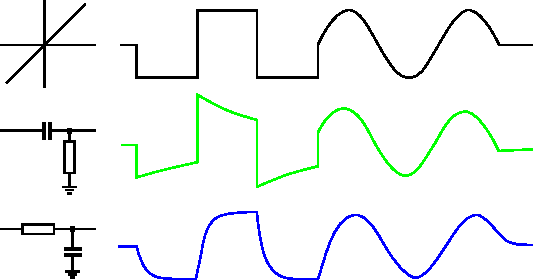
\includegraphics[width=.4\linewidth]{imgs/fourier/distortion.pdf}
  \end{center}
  
  \begin{block}{Phase distortion}
    Let a system of frequency response 
    $$\tilde H(w)=|H(w)|e^{j\phi(w)}$$

  We can deduce that for 
\begin{align*}
x(t)&=\cos(\omega t)\\
y(t)&=|\tilde H(\omega)| \cos(\omega t+ \phi(\omega))=|\tilde H(\omega)| \cos(\omega (t+ \phi(\omega)/\omega))
\end{align*}
The delay $\phi(\omega)/\omega$ is also called  \textbf{propagation time} of \textbf{frequency delay}.  For it to be independent from frequency it is necessary that
\begin{displaymath}
\frac{\phi(\omega)}{\omega}=cte=\tau\quad \rightarrow \quad \phi(\omega)=\omega\tau
\end{displaymath}
  \end{block}

  \frametitle{Ideal low pass filter}

  \begin{block}{Definition}
    \begin{itemize}
    \item The ideal low-pass filter is often a theoretical object in signal processing.
    \item Perfect to use when the noise and signal have non-overlapping spectra.
    \item The frequency response of the ideal filter is 
$$
H(f)= \left \{ 
\begin{array}{ll}
1 & \text{ if } |f| < f_c \\
0 & \text{ else} 
\end{array}
\right.
$$
where $f_c$ is the cutoff frequency.
\item The impulse response of the filter is %\pause
\begin{equation*}
  h(t)={2f_c\frac{\sin(2\pi f_c t)}{2\pi f_ct}=2f_c\text{sinc}(2\pi f_ct)}
\end{equation*}
    \end{itemize}
  \end{block}
\vspace{-5mm}
  \begin{block}{Realizable filter}
    \begin{itemize}
    \item A realizable temporal filter is \textbf{causal} and \textbf{stable} (absolute integrable).
    \item Ideal filter is neither of those and cannot be used for 1D (time) filtering.
    \item For images (2D) causality is not necessary.
    \end{itemize}
  \end{block}


  \frametitle{Filter design}
  
  \begin{block}{Real filter}
    \begin{itemize}
    \item Ideal filters are non causal and cannot be implemented in practice .
    \item We search for an approximation of the ideal filter.
    \item the approximation has to respect \textbf{constraints} (Gabarit in french).
    \end{itemize}
  \end{block}


  \begin{block}{Constraints of a filter}

\begin{columns}[T]
  \begin{column}%{5cm}
%\vspace{-5mm}
       \begin{center}
 % 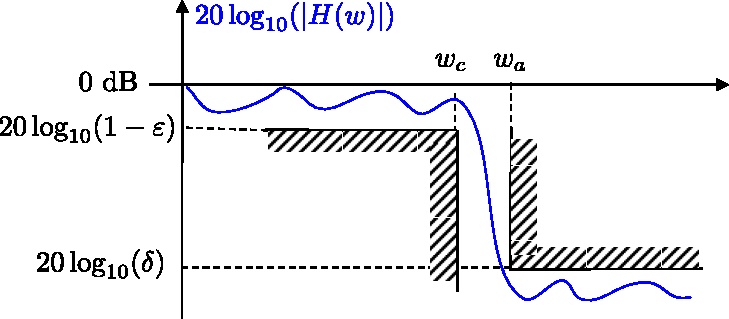
\includegraphics[width=1.1\columnwidth]{imgs/gabarit3}
\end{center}
  \end{column}%\vspace{-5mm}
  \begin{column}%{6cm}%\vspace{-5mm}
    \begin{block}{Parameters:}
      \begin{itemize}
      \item Bandwidth $BP$ and rejected band
      \item Oscillations :
        \begin{itemize}
        \item $\varepsilon$ in passing bandwidth
        \item $\delta$ in attenuated bandwidth
        \end{itemize}
      \end{itemize}\vspace{7mm}
    \end{block}

  \end{column}
\end{columns}
 The constraints define the area that are acceptable for a given application.
  \end{block}

\subsection{Modulation}
\label{sec:modulation}

\subsection{Fourier optics}
\label{sec:}